 \chapter{Tracking Adaptive Performance Models using Dynamic Clustering of User Classes}
 \label{ch:estimation} 
%\begin{center}
%\textbf{This chapter contains material from Ghanbari et al. \cite{hamoun_ghanbari_tuning}}.
%\end{center}

  This dissertation uses a model to project the state of the system under different actions. 
	%  The modelling enables the controller to project the system's behaviour and state under different actions.  
 To do this projection, one needs to have the current state of the system in terms of the model elements. The objective of an estimator is to describe the system in terms of a given parametric model. This identification process includes finding or estimating the parameters of the model using the data obtained from the system, in an ongoing fashion.  
 
 In our case, the model corresponds to the cloud and the service instances, which run within the cloud. Thus, the identification mostly corresponds to the estimation of workload intensities (the number of users and the think times in a closed workload case and the arrival rate in an open workload case) and the service demands which are treated as hidden parameters of the model
\cite{
rolia_parameter_1995,
rolia_correlating_1998,
courtois_using_2000,
pacifici_cpu_2008,
zhang_regression-based_2007,
zhang_workload_2002,
liu_parameter_2006,
gmach_workload_2007,
gmach_capacity_2007}. 

  The estimation is carried out using the measured parameters of the system such as device utilizations ($U_{h,k}$), or class throughputs ($X_{c}$), and response times($R_c$), if available.
     For each measurement metric obtained from the monitoring subsystem, we have one or more relations according to the queuing theory. We use these relations in the context of the Kalman filtering approach.  
		
		
	  % --------------------------------------------------
  \section{Bayesian Estimation of Hidden LQN Parameters Using Extended Kalman Filter Estimator}    
  \label{sec:bayesian-estimation}  
   In the Bayesian approach, the probability estimate for a hypothesis is updated as additional evidence is learned; this makes Bayesian approach a good fit for estimation tasks on sequential data. One can look at performance data as a sequence of measurements, where the unknown performance parameters are changing parameters to be estimated from observations \cite{woodside_use_2005,xu_performance_2005,zheng_tracking_2005}.
   
   All parameters are taken as latent variables. So it is assumed that the parameters distributions also vary over time, and there exists a \textit{state-space model} that specifies the dynamics of latent variables and the relation among the latent variables and the observations. 
Assuming that one knows the state and the measurement noise covariance structures, one can estimate the model parameters by solving the associated optimization. 
Assuming Gaussian noise, subject to model and domain constraints, the estimation problem can be described using the following optimization expression:  
    % \footnote{Note that with the assumption that $x$ has multivariate Gaussian distribution, at any given point in time $\hat{x}_t$ and $P_t$ fully present the state vector distribution. This also applies to $\hat{x}_0$ and $P_0$.}
  \footnote{Note that, determining the optimal parameter estimates cannot be done using a weighted least squares optimization of the measurement residuals (i.e. $y_t - h(x_t)$) with respect to the model parameters $\theta$, since the process equation in the model is non-deterministic.} 
  
  
  
\begin{align*} 
 %  \label{eq:mhe-optimization} 
 % \nonumber \\     
 \underset{x_0,...,x_T}{\text{minimize }}  
   &  (x_0-\hat{x}_0)P^{-1}(x_0-\hat{x}_0)
 	 + \sum_{t'=0}^{T-1} w^T_t Q^{-1}_t w_t 
	 + \sum_{t'=0}^{T}  v^T_t R^{-1}_t v_t \nonumber  \\ 
    \text{subject to:} \nonumber \\   
    & \hat{x}_t=[\overrightarrow{\hat{d}_t},\overrightarrow{\hat{N}_t},\overrightarrow{\hat{Z}_t}]^T  \nonumber \\  
    & u_t=[\overrightarrow{\tilde{d}_t},\overrightarrow{\tilde{N}_t},\overrightarrow{\tilde{Z}_t},\overrightarrow{\tilde{\Omega}_t}, \overrightarrow{\tilde{\rho}_t}]^T  \nonumber \\   
    & z_t=[\overrightarrow{R_t},\overrightarrow{U_{h,k',t'}},\overrightarrow{X_{s,h,t'}}]^T  \nonumber \\   
    & x_{t + 1} = x_t+w_t \nonumber \\     
    & z_t = LQM_{\tilde{x}_t}(\hat{x}_t)+v_t  \nonumber \\
    &  d_{c,s,h,t}>0  && \text{  for each $c$,$s$,$h$,$t$}  \nonumber \\  
    &  0<U_{h,t}< 1 && \text{ for each $h$, $k$} \nonumber
\end{align*} 
%% One of the benefits of this approach is the fact that we can specify dynamics of the state transition explicitly. 
where 
 $t$ denotes the discrete time. 
 $\tilde{x}_t$ is used to represent the known portion of $LQM$ parameters such as multiplicity of resources at time $t$. In other words, every value of $\tilde{x}_t$ defines a function of $x_t$, denoted by $LQM_{\tilde{x}_t}$. 
 $w_t$ is the process noise with a normal distribution, zero mean, and the covariance of $Q_t$ (i.e. $N(0,Q_t)$),  
 $v_t$ is the observation noise with a normal distribution, zero mean, and the covariance of $R_t$ (i.e. $N(0,R_t)$).  
 $x_t$ is the state to be estimated, composed of unobserved LQM parameters, with the mean of $\hat{x}_t$ and covariance matrix of $P_t$ (i.e. $N(\hat{x}_t,P_t)$).
 %For example, for two classes $\{c_1,c_2\}$, one service $\{s_1\}$ and one host $\{h_1\}$, the state can be:  
   %\begin{align} 
  %x_t=[d_{c1,s1,h1,t'},d_{c2,s1,h1,t'}, X_{c1,s1,h1,t'},X_{c2,s1,h1,t'}]^T  \label{eq:two-class-state-vec}  
 %\end{align}  
 %$z_t$ is the observed data vector that is output of the model.  
 $z_t$ is the vector representing the measured performance.  
 $LQM_{\tilde{x}_t}(\hat{x}_t)$ is, in this case, the observation model based on the queuing theory formulas \ref{eq:queuing-model1} to \ref{eq:queuing-model4} and it is non-linear with respect to the state vector.   
  % For example, in case of missing throughput values per classes, the state vector becomes: $x_t=\{D_{s,k',t'}\} \cup \{X_{c,s,t'}\}$.   

%\begin{figure}
	%\centering		
	%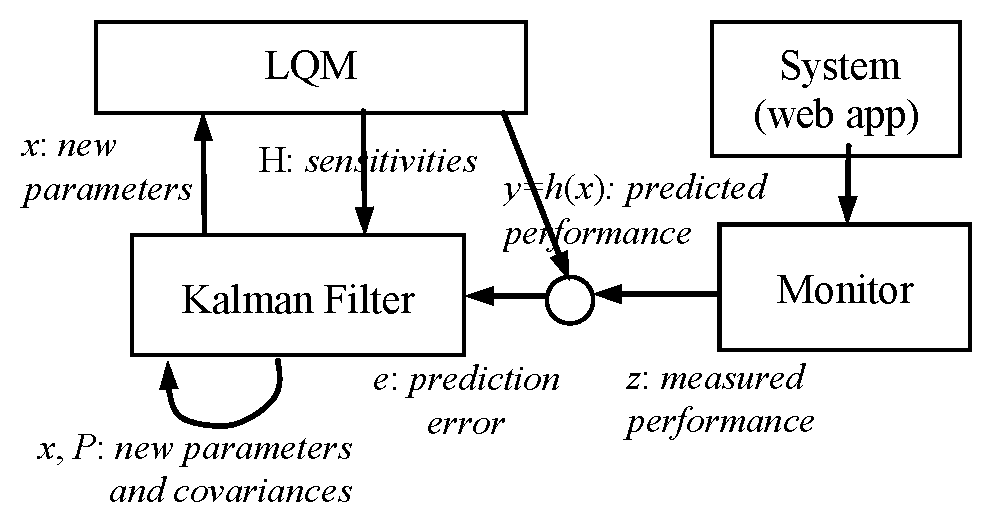
\includegraphics[width=0.8\textwidth]{image/image-tracking-structure.eps}  
	%\caption{Architecture of feedback based estimation using the extended Kalman Filter.} 
	%\label{fig:fig1}
%\end{figure}  
 The solution to the above optimization can be derived by an Extended Kalman Filter (EKF) \cite{zheng_tracking_2005}, a variant of the Kalman filter \cite{brookner_tracking_1998}. 
%Figure \ref{fig:fig1} depicts the architecture of this extended Kalman filter. Let $x$ and $z$ be vectors representing the parameters and measured performance, respectively. The model maps $x$ to an output vector $y$ (i.e., $y=h(x)$) which represents the predicted performance. The filter then estimates $x$ (which is not directly measurable) based on the observed performance $z$. 

 Assumed prior knowledge of the filter includes distribution of the initial state, and process and measurement noise structures: 
\begin{equation}\label{eq:filter-initial-state}\begin{split}
  \hat{x}_0  \\ %. I added the hat later on
  P_0&=E[(x-\hat{x}_0)(x-\hat{x}_0)^T]  \\
  Q_t &= E[w_t w_t^T]  \\
  R_t &= E[v_t v_t^T]  \\ 
 \end{split}\end{equation}   
 where
   $\hat{x}_0$ is the initial estimate,
    $P_0$ is the initial error covariance matrix, and 
   $Q$ and $R$ are the covariance matrices for the process and measurement noise, respectively.
  
%\begin{minipage}{\linewidth} 
The filter computations are recursive, beginning from an initial estimate $\hat{x}_0$, and an initial error covariance matrix $P_0$.
Each recursive step can be summarized as follows: 
\begin{enumerate}
\item  The core filter calculation is the update of the state estimate $\hat{x}_t$ and error covariance estimate $P_t$ by the linear feedback equation:
 \begin{align} 
& H_{t} = \left . \frac{\partial h}{\partial x } \right \vert_{\hat{x}_t^-,u} \\
& K_t  =P_t^- H_t^T (H_t P_t^- H_t^T+ V_t )^{-1} \\ 
& e_t   = z_t  - LQM_{\tilde{x}_t}(\hat{x}_t^-)  \label{eq:observation-error} \\  
& \hat{x}_t = \hat{x}_t^- + K_t e_t   \\
& P_t=P_t^- - K_t H_t P_t^-       
 \end{align}
\item The filter then projects the state estimate $\hat{x}_t$ and the error covariance matrix $P_t$ forward one step:  \begin{align}
  % \hat{x}_{k+1} = F(\hat{x}_t,u_t) 
 & P_{t+1}^-  = AP_tA^T+Q \\
 & \hat{x}_{t+1}^-=\hat{x}_t
 \end{align} 
\end{enumerate}
%\end{minipage}

 Here, $e_t$ denotes the prediction error vector obtained from the current modelled and observed output vectors ($LQM_u(\hat{x}_t^-)$ and $z_t$ respectively), and $P_t^- $ denotes the value of $P_t$  at time $t$ given measurements up to time $t-1$ (i.e. $P_{t|t-1}$).  
 $H_t$ is the matrix of sensitivity values or partial derivatives of the model function (i.e. $LQM_{\tilde{x}_t}(x_t)$) with respect to the parameters at their current values $x_{k}$,  whose $j$th column is the derivative of $LQM_{\tilde{x}_t}(x)$ with respect to $x_j$. 
 Essentially, this Extended Kalman filter (EKF) [25] linearizes $LQM_{\tilde{x}_t}(x_{t-1})$ by a first order Taylor series around the state estimate and does not take linearization errors into account. 

 Also note that here we assumed the process model chosen to describe the state is a ``random walk."  In this scheme the system state $x_t$ (here demand and workload) is assumed to evolve due to random drift $w$ as: $x_{k+1}= x_t+ w_t$. This means that a minimal assumption is made during the estimation of hidden parameters of this model: that the covariance matrix for $w_t$ is known (we denote it by $Q_t$). 
 Usually the covariance matrix is diagonal since workload components (number of users and think time) and user demands are assumed to change independently. The values are sometimes set according to $Q_{i,i} = \alpha  x_0(i)$, where $x_0(i)$ is the initial value of the $i$-th state variable to be estimated, and $\alpha$ is the ratio of expected changes for $x_i$'s,  (e.g. 0.02) with respect to their initial values.   

 The optimality and the convergence properties of the Kalman filter depend on the way the functions are linearized around the current estimate of x.   
  % Even the simple throughput and utilization measurement case solved with LSE, in the presence of missing throughput-per-class measurements, becomes non-linear with respect to the state vector. For example, assuming state vector  $x_t=[d_{c1,h1,t'},d_{c2,h1,t'}, X_{c1,h1,t'},X_{c2,h1,t'}]^T $, the utilization law $U_{h,t'}=\sum_c X_{c,h,t'} D_{c,h,t'}$, which is linear with respect to $c_{c,h,t'}$,  is non-linear with respect to state vector $x_t$:  $ U_t(x) = x_{1,t'}x_{3,t'}+x_{2,t'}x_{4,t'} $.   
	% --------------------%
	% these are just added
		The approximated $H$ matrix and the equations of the filter depend on the following three factors: 


  \textbf{The required estimates.} 
  The main estimates to be discovered are the service demands, and most of the time, the user population ($N_c$) and think time ($Z_c$) of each class. In this chapter, we assume that each service replica is identified by a subscript $j=1...J$ which summarizes a tuple $(s,h)$  (see the chapter 2). In other words, a replica $j$ is implicitly associated with a host $h$ and a service $s$. So a demand $d_{c,s,h,k}$ (introduced in the chapter 2) is re-written as $d_{c,j,k}$.  $d_{c,j,k}$ represents the service demand of a class $c$ at a replica $j$, on a hardware resource $k$. This is done to associate the variables exclusively to the unknowns and reduce the total number of variables. If there is no replica of a service $s$ placed on a host $h$, there will not be any variable $d_{c,j,k}$ defined for its estimated value. Note that the Kalman filter does not provide a way to enforce the equality constraints such as $d_{c,s,h,k}=0$ during estimation. So, one needs to substitute such variables with the associated constants.   

  \textbf{The measured parameters.}
     Usually the throughput of each class of users ($X_c$) can be easily obtained. The mean utilization of each resource type $k$ (e.g. CPU, disk, and network) on each host $h$ ($U_{h,k}$) and the mean response time for each user class ($R_{c}$) are also usually available. % for one req 

     \textbf{The missing data items.} On certain occasions, a subset of metrics from a subset of servers might be missing. For example, it is usually not feasible to get response time metrics from individual service replicas ($R_{c,j}$) without code manipulation or instrumentation. These missing data items are also treated as variables in our model.  
% Assume all the information captured from the real system, is summarized in a measurement vector $z$.  In the perfect information case $z$ would be: $z_t=[R_{h,s,t'},...,U_{h,k,t'},...,X_{s,h,t'}]$. 
%where $J=\left\vert{\{j=(s,h)|\theta_{s,h}\neq 0\}\right\vert}=\text{count}(\theta_{s,h}\neq 0)$ 


	 
\section{Dynamic Clustering of User Classes}  
  An important issue in using the Kalman filtering approach is convergence. The necessary and sufficient condition is given by the identifiability condition \cite{tanizaki_nonlinear_1996,wan_unscented_2000,welch_introduction_1995}. The convergence requires that at minimum, we have more measured parameters than estimated state parameters: i.e., 
   \begin{align}  
   \text{dim}(x) \leq \text{dim}(y)    \label{eq:identifiability}
    \end{align}    

 As we know, the estimated parameters might include:   
  (i) the demand of each class, on each service replica, on each resource ($d_{c,j,k}$), 
  (ii) the mean think time for each class ($Z_c$), 
 (iii) the number of users in each class ($N_c$).  
 
	  
 Thus $\text{dim}(x)$, based on the number of classes ($C$), the types of resources available in each server ($K$), and the number of service replicas in the deployment ($J$) is as follows\footnote{The dot sign was used to represent the multiplication.}:                
 \[ \text{dim}(x)=C\cdot J\cdot K +  C + C = C\cdot (J\cdot K+2) \]
 
In the case of $K=1$ (i.e. only one resource type), we have: \[\text{dim}(x)=C\cdot (J+2)\] 

 Note that in reality, the services can be classified into two kinds: the application-specific services, and the generic services.
   The relationship between classes and application specific services is a sparse one; meaning that there is a small number of application services used exclusively by each class of users. On the other hand, the relationship between the classes and the generic services is very dense because almost all the classes make use of some primary core services. 
   This sparsity and uniqueness, which constitutes an N-to-1 relationship between application services and classes, is a great help when it comes to estimation of the demands on user services. 
 In a sparse deployment, the term $C\cdot J\cdot K$ will be hugely decreased due to the fact that not every class $c$ makes use of a service replica $j$. 
 
  The measured parameters are most likely the mean response time and throughput of each class and the utilization of each server. If we also have a number of other measurements denoted by $\phi$ (for example the response time of each class at a service replica gives us another $C$ measurements) it results into: \[ \text{dim}(y) = \phi+2C + H\]  and the identifiability condition \ref{eq:identifiability} reduces to:
 \begin{align}  
 & \phi+2C + H \geq  C\cdot (J+2)  \\  
 & H+\phi \geq C\cdot J \\ 
  & C \leq H/J+\phi/J
  \end{align}    
   thus $\text{dim}(x)> \text{dim}(y)$, if $C$ is reduced to at least $(H+\phi)/J$. 
 Note that replicas are at least equal to the utilized hosts ($H\leq J|U_h>0$). So, the main factor is the number of extra measurements at the service replicas (i.e. $\phi$).  
For each additional class beyond $H/J$, we need an additional $J$ measurements. 
This linearly increases the monitoring overhead.
We should, therefore, keep the number of classes small, if possible. 

%\subsection{aggregation semantics}     
%Suppose the tensor $d$ assigns a value to every triple $<c,s,k>$. 
% Remember that $d_{c,s,k}=V_{c,s}D_{s,k}$. In order to make the number of unknowns smaller than dimensions of the tensor $d$ must be aggregated into a set of clusters.     
%In the rest of this section we propose a combination of clustering algorithm and bayesian method for effective grouping of classes. The clustering uses the K-means algorithm. 
%convergence: start from 1 class and go up until it does not converge because it is too many unknowns 
%Accuracy: how to measure accuracy? from the optimization. Every number of clusters corresponds to a different cost function (see \ref{eq:mhe-cost-function} ) and consequently different minimization problem, and different optimal trade-off curve.  Thus the measure of accuracy is actually the tradeoff curve or the $J$ that is achieved. f  
%Suppose there are $L$ services (i.e. $i=1,\dots,L$) in the system. 
%Let $R_{c(i)}$ be the predicted mean response time of class $c(i)$ requests. 
% we would like to have $C^0$ initial clusters in the system (i.e. $c=1,\dots,C^0$)
%

%\subsection{Dynamic Clustering Algorithm}
%\label{sec:dynamic-clustering-algorithm} 
In this section, we first discuss the modelling error due to clustering and then present an algorithm to determine the best choice of the number of clusters $C$ and the grouping of classes into these clusters.

\subsection{Modeling Error} 
\label{sec:modeling-error} 
Suppose the original $C$ classes (i.e. $c=1,\dots,C$) are reduced to $C'$ classes (i.e. $c'=1,\dots,C'$), and $c'=\psi(c)$ where $\psi$ is the function that maps the class $c$ in the original model to $c'$ in the new model. Let $R_{\psi(c)}$ be the predicted mean response time of class $\psi(c)$ requests. For the case of no clustering (i.e., each class in the original model is treated as a separate class in the new model), let ${R(C)}_c$ be the mean measured response time of requests for the original class $c$. Then a modeling error measure $E(C')$ for a new model with $C'$ classes is given by: 
\begin{align}    
	E_\psi(C')=\sqrt{\frac{1}{C}\sum^C_{c=1}{{\left(\frac{{R(C)}_c-\ R_{\psi\left(c\right)}}{{R(C)}_c}\right)}^2}}
		%=\textcolor{red}{\boldsymbol{\left|\left|\boldsymbol{\frac{R(C)-R_\psi}{R(C)}}\right|\right|}}
		\label{eq:modeling-error}     
\end{align}  

The hypothesis is that the error $E(C')$ tends to decrease when the number of clusters is increased. However, finding the clusters and the multi-class performance model associated with the clusters is complex, as $E$ is also a measure of how well the results from the filter and the model fit the measured data.




\subsection{Dynamic Clustering Algorithm} 
\label{sec:dynamic-clustering-algorithm-sub} 
Our classification algorithm is shown in Algorithm \ref{algorithm-estimation}.  Inputs to this algorithm are the LQM, a measurement vector $z$ and an error threshold $A$. The vector $z$ can include workload elements $\overrightarrow{\lambda_c}$ or $(\overrightarrow{N_c},\overrightarrow{Z_c})$, the measured response time $\overrightarrow{R^\text{m}_c}$ and throughputs $\overrightarrow{X^\text{m}_c}$, and the total utilization of the servers $\overrightarrow{U_h}$. The algorithm generates the best values of the number of classes (i.e. $C'$) for the new model, the grouping of original classes into these  classes (i.e. function $\psi$), and the service demand estimates for the service replicas (i.e. $d_{c',j,k}$, $\forall j\in\{1, \dots,J\}$, $\forall c'\in\{1, \dots,C'\}$, $\forall k\in\{1, \dots,k\}$).


\begin{algorithm}
	\small
	\SetAlgoVlined
	\SetKwInOut{Input}{input}
	\SetKwInOut{Output}{output}
	\SetKwInOut{Initialize}{initialize}
       \SetAlFnt{\tiny}

\Input{LQM, $z$, $A$}

\Output{The best choice of the number of clusters $C'$, aggregated demand ($d_{c',j,k}$) and mapping of old classes to new ones $c'=\psi(c)$. }

\BlankLine
$\{d_{c,j,k}\} \gets$ Estimate $d_{c,j,k}$, the service demand of class $c$, service replica $j=(s,h)$, at resource type $k$, from measurement data ($\forall j=(s,h)\in\{1, \dots,J\}$, $\forall c\in\{1, \dots,C\}$, $\forall k\in\{1, \dots,k\}$) using the model with no clustering; and set $C' = 1$.
\BlankLine 

\Repeat{$E(C') < A$}{
$\psi_{\{d_{c,j,k}\},C'} \gets$ Cluster the services based on the $d_{c,j,k}$'s into $C'$ clusters. 


$\{d_{c',j,k}\} ,\{R_{c'}\} \gets$ Estimate the parameters
$d_{c',j,k}$, the service demand of class $c'$ at replica $j$, at resource type $k$; solve the LQM with $C'$ classes and obtain results for $R_{c'}$, the mean response time of class $c'$ ($\forall j\in\{1, \dots,J\}$, $\forall c'\in\{1, \dots,C'\}$, $\forall k\in\{1, \dots,k\}$). 
\BlankLine

$E(C') \gets$ Calculate the modelling error  \BlankLine 

%If $E(C') > A$, then increase $C'$ by $1$ and go to Step 2. 
Increase $C'$ by $1$
\BlankLine 
}
Return $C'$, $\psi$ the original classes $c'$ associated with each cluster $c'$, and
$d_{c',j,k}$ ($\forall j\in\{1,\dots,J\}$, $\forall c'\in\{1,...,C'\}$, $\forall k\in\{1, \dots,k\}$ ) 
\BlankLine

\caption[The algorithm for estimation of service demands and clustering of user classes.]{The algorithm for estimation of service demands and clustering of user classes.}
\label{algorithm-estimation}
\end{algorithm}

In our investigation, the workload is time varying. The autonomic control loop is executed at regular intervals. If the modeling error of the existing grouping configuration is less than $A$, only the regular estimation is performed using the Kalman filter. On the other hand, if modelling error is greater than $A$, our clustering algorithm is invoked to obtain a new clustering of classes such that the modelling error becomes less than $A$ (see algorithm \ref{algorithm-estimation}). 

The clustering algorithm starts by estimating the service demands of all the service replicas from the measured response times using the original model with no clustering (Step 1). The estimation at this step is done by using either an Extended Kalman filter or the linear or non-linear least squares methods described in chapter 2.
Note that this is different from the estimation that is done at each step. The purpose of this estimation is solely for clustering the classes. 
If an EKF is used, the convergence criteria should be considered, and extra measurements should be used if necessary.  One can use the least squares method, taking the demands constant over the past few steps (moving horizon estimation format or MHE) to avoid the need for extra measurements. The necessary condition for this case is to have the estimation horizon wide enough to contain enough data points for the least squares method.   

In Step 3, the K-means clustering algorithm \cite{kaufman_finding_1990,likas_global_2003} is used to perform an unsupervised grouping of the service demands. K-means has low complexity and is adaptable to the continuous nature of our problem. Moreover, it is able to detect clusters in an efficient way, which does not require computing the distance of all the points to one another. K-means takes as input the number of distinct clusters to generate ($C'$) and will determine the size and members of the clusters (mapping between the classes and the clusters) based on the demands. 

The modeling error $E(C')$ is calculated at Step 5 using the $R_{c'}$, that was obtained in Step 4. If $E(C')\le A$, the algorithm terminates and returns (i) the best choice of the number of clusters, $C'$, (ii) the classes assigned to each of the $C$ classes, $\psi$, and (iii) the estimated service parameters for the different classes $d_{c',j,k}$ (see Step 7). 
 If the modelling error $E(C')$ is larger than the acceptable error $A$ (i.e. due to a gradual change in service demands over time) the algorithm increases the number of clusters and performs another iteration. Steps 3, 4 and 5 are then repeated to compute $E(C')$ for the new number of clusters. Note that a larger number of clusters would increase the measurement overhead and the computational cost of estimation, but it will decrease $E(C')$. 

\section{Experiment 1: TPC-W benchmark and FIFA98 workload}    
To show the applicability of the method, we performed our first experiment on the estimation of service demands of the TPC-W benchmark \cite{garcia2003tpc} implementation. We deployed the Java implementation of TPC-W \cite{volker_turau_tpc-w_????} with some modification, on a cluster of four Tomcat web servers and one single MySQL database server, with Linux as the operating system. 

TPC-W is an e-commerce web application composed of 14 URLs, namely 'admin confirmation, admin request, bestsellers, buy confirm, buy request, registration, home, new product, order display, order inquiry, product detail, search request, search result, shopping cart'.  Each of the URLs has a different service demands on web and database servers. 

The application also comes with a workload generator, which takes as input: (i) the number of users over time and (ii) a Customer Behavior Model Graph (CBMG), given to the workload generator as  a transition probability  matrix of a Markov chain. This workload is generated using Emulated Browsers (EB) whose behaviour and navigation is controlled by the Markov chain.  

The number of users over time are derived from FIFA98's workload \cite{arlitt_workload_2000}\footnote{The reason we chose FIFA98's workload over some other workloads commonly used in computing systems performance community (e.g. Google Workload Traces \cite{reiss2011google}) is that the workload includes very detailed information about access patterns of a web application by online users. Basically the workload is the detailed log of Apache web servers.
Google Workload Traces is mostly concerned with the amount of time it takes it Google cloud to complete a job and the performance of the scheduling. The trace also includes hardware level information about the resource usage on the physical machines. }.
This workload reflects variations that servers might experience at runtime. We picked a portion of the day 21's workload (see Figure 6), extracted the web pages, lowered the number of requests by the factor of 2 (to factor in our smaller scale deployment topology), and finally used Little's law \cite{little1961proof}  (i.e. $N=X(R+Z)$) to convert the obtained throughput ($X$) to the number of users ($N$) and think time ($Z$) used by the emulated browsers of TPC-W. We assumed that the FIFA98 website had maintained the same response time over the sampling period. % We then used the obtained number of users to the TPC-W benchmark using equal mix of buying, browsing, and ordering scenarios. 

 \begin{figure}[hp]
	\centering
		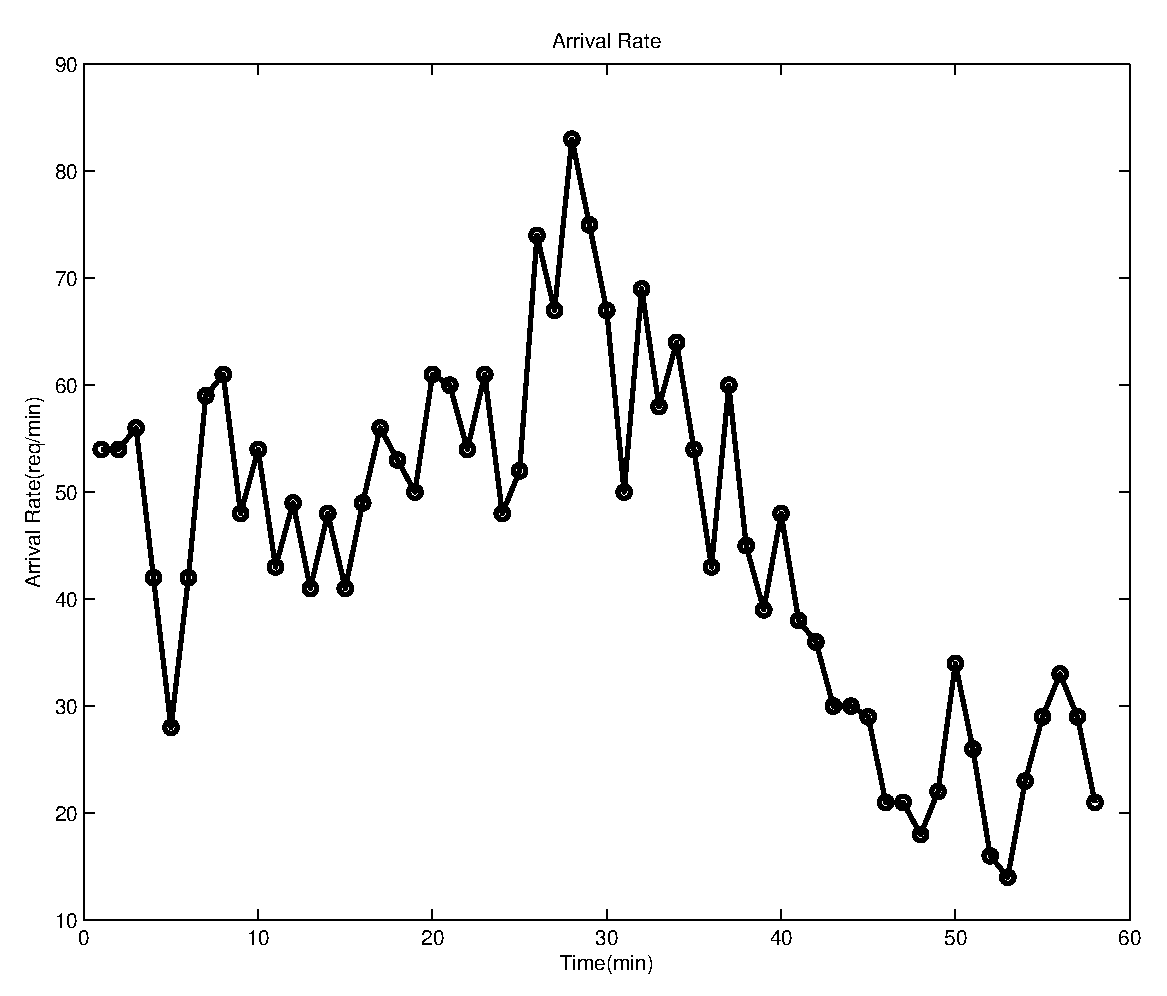
\includegraphics[width=0.7\textwidth]{image/workload-arr-rate.eps}
	\caption[FIFA98 workload, day 21, over an hour, used in demonstration of the estimation algorithm.]{FIFA98 workload, day 21, over an hour.}
	\label{fig:fig2}
\end{figure}
For obtaining data, we monitored one of the web servers and the database and logged data collected from one of the web servers and the database; these included: response times, throughputs, and utilizations. Each sample represented a minute of work, and the total length of the experiment was 1 hour resulting into 60 samples.

 \textbf{Estimation.} 
    The application was modeled as two services, web and database. Each service only has one replica placed on a separate server. We also took the users accessing the system through each individual URL as a class of users. 
    
		The average number of visits to web and database services are different for each class depending on the CBMG. This makes the average web and database service demands for each URL different, and subject to estimation. This leaves us with 28 parameters to estimate, 14 web service demands $d_{c,\text{w}}$ and 14 database service demands $d_{c,\text{db}}$. Note that there is only one service replica for each of the services in the system, each installed on a different host.
		
		The monitored metrics include the throughput and response time of each class (28 measurements) and the utilization of each server (2 measurements). Since number of measurements is already more than the number of unknowns (28 versus 30), the convergence criterion is met even with no clustering.

		Figure \ref{fig:estimated-demands-casestudy1} represents the estimated service demands for 13 classes for the web service. One service demand is removed from the diagram to increase the clarity. 
 \begin{figure}[htbp]
	\centering
	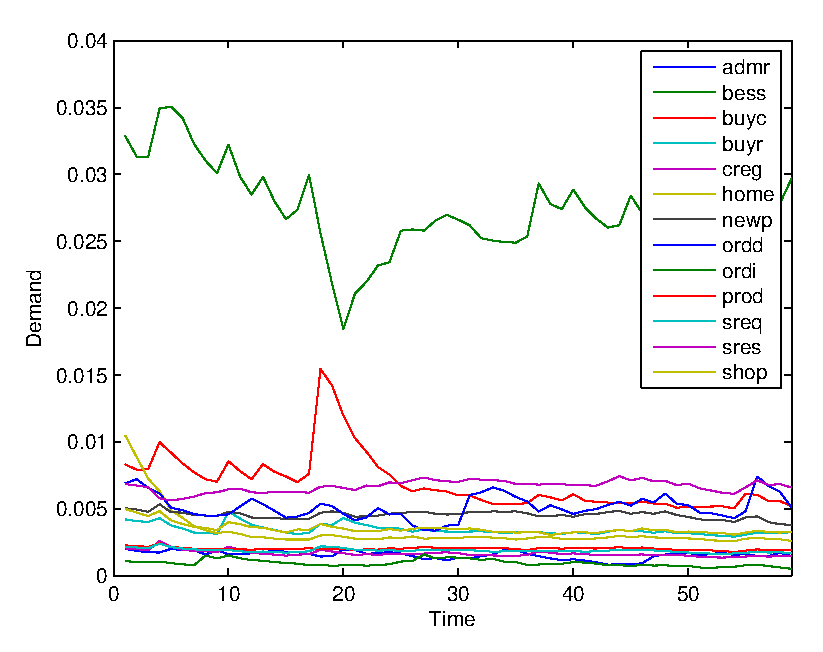
\includegraphics[width=0.7\textwidth]{image/demand13_estimated_kamlan.eps}
	\caption[A sample example of estimated service demand of 14 classes on a single service.]{Estimated service demand for 14 URLs on Web server service.}
	\label{fig:estimated-demands-casestudy1}
\end{figure}
Note that in the diagram the demands do not change frequently. We suspected that this is mainly because (i) the workload is unable to fully saturate the system or (ii) the combination of workload mixes are the same.
      
  Our analysis on this experiment had three parts. First, we ran the algorithm statically with a different number of clusters and measured the modelling error. In our evaluation, we used an expanded definition of the modeling error metric given by its average over the duration of the experiment (from $1$ to $T$): 
 \begin{align} 
 E=\frac{\sum^T_{t=1}{E(C')_{t}}}{T} 
  \end{align} 
where $t$ ranges over the estimation steps. $E(C)$ is the modelling error defined in equation \ref{eq:modeling-error} and $T$ is the number of estimation steps. 
\begin{figure}[htbp]
	\centering
	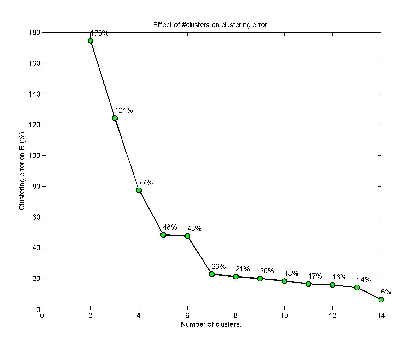
\includegraphics[width=0.7\textwidth]{image/modeling-error-vs-num-cluster.eps}
	\caption[The relationship between the modeling error and the number of clusters.]{Modeling error decreases with the number of clusters.}
	\label{fig:modeling-error-decreases}
\end{figure}

 As we expected, the error decreased while we increased the number of clusters (See Figure \ref{fig:modeling-error-decreases}). The experiment also shows that modelling the system with one or even two classes introduces a large modelling error and that modelling with an intermediate number of classes (8, for example) might give us an acceptable modelling error. 
\begin{figure}[htbp]
	\centering
	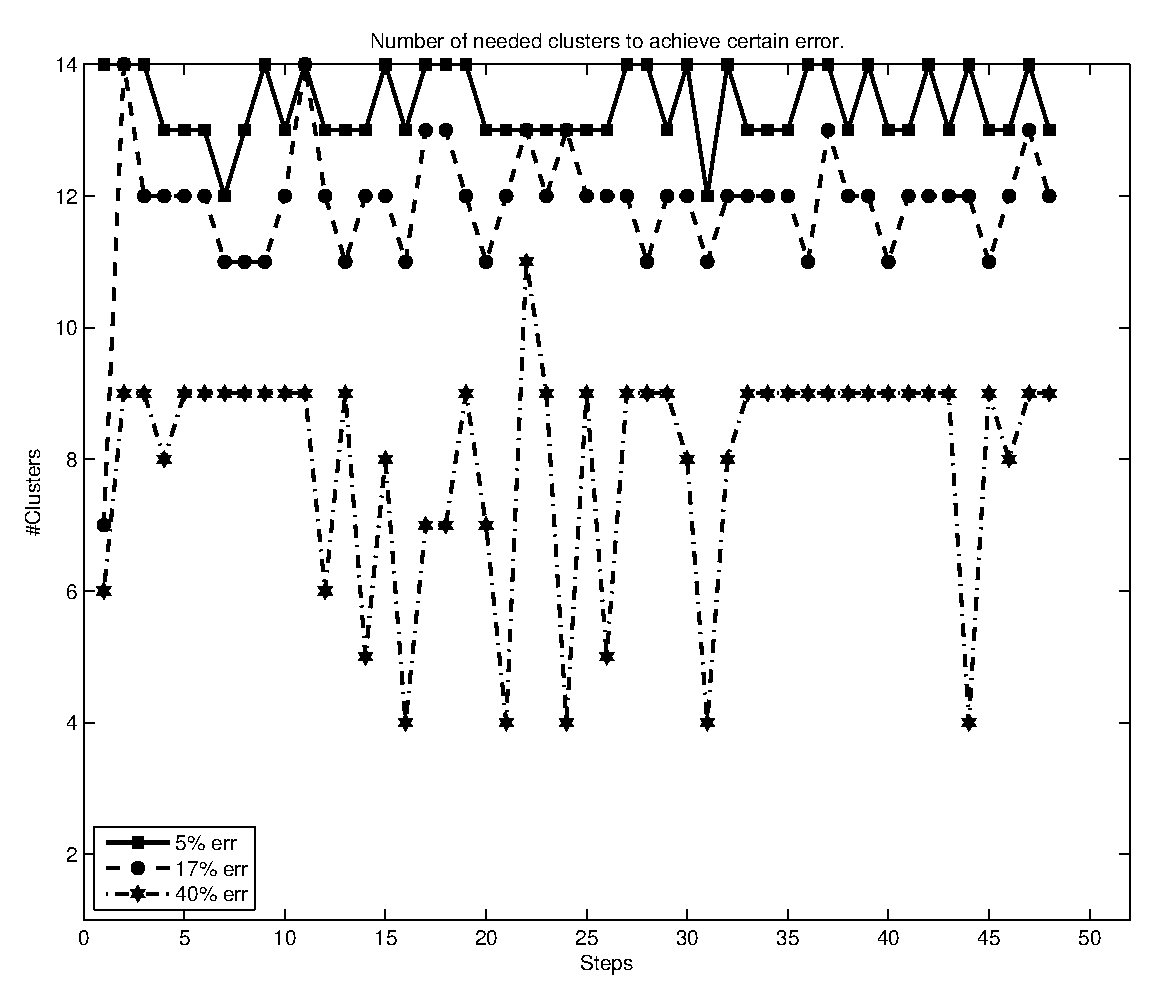
\includegraphics[width=0.7\textwidth]{image/cluster_num_by_error.eps} 
	\caption[ The minimum number of clusters, dynamically adjusted, to reach a certain modeling error.]{The minimal number of clusters needed to reach a specific modeling error threshold.  We can reach 40\% and 17\% error, consecutively using 9 and 12 clusters on average. In order to reach 5\% error, we have to perform full clustering.}
	\label{fig:minimal-number-needed-clusters}      
\end{figure}

In the second part, we applied our estimation and clustering algorithm to find the minimal number of needed clusters to reach a certain modelling error. The algorithm is applied at each sampling period and, as a result, the clusters change dynamically. As Figure \ref{fig:minimal-number-needed-clusters} shows, we can reach 17\% error using between 7 and 12 clusters for the duration of the experiment. For a modelling error less than 40\% we need 9 clusters on average. In order to reach 5\%, there are sampling periods in which we need maximum number of classes, which is 14.

In the third part of the analysis, we observed the correlation between the \textit{within cluster sum-of-squares} (WCSS) for demands and the modelling error achieved using the estimation and clustering algorithm. We chose 140 different groupings. For each number of clusters, we generated 10 random combinations. This let us navigate all possible WCSS's that could result from different groupings. Figure \ref{fig:cluster-sum-of-squares} shows that, on average we experienced a larger modelling error for the clusters with higher WCSS errors. In other words, the modelling error is minimized, whenever the WCSS is minimized. As a result, our assumption is validated since K-means is exactly the algorithm to minimize the WCSS. 
\begin{figure}[h]
	\centering
	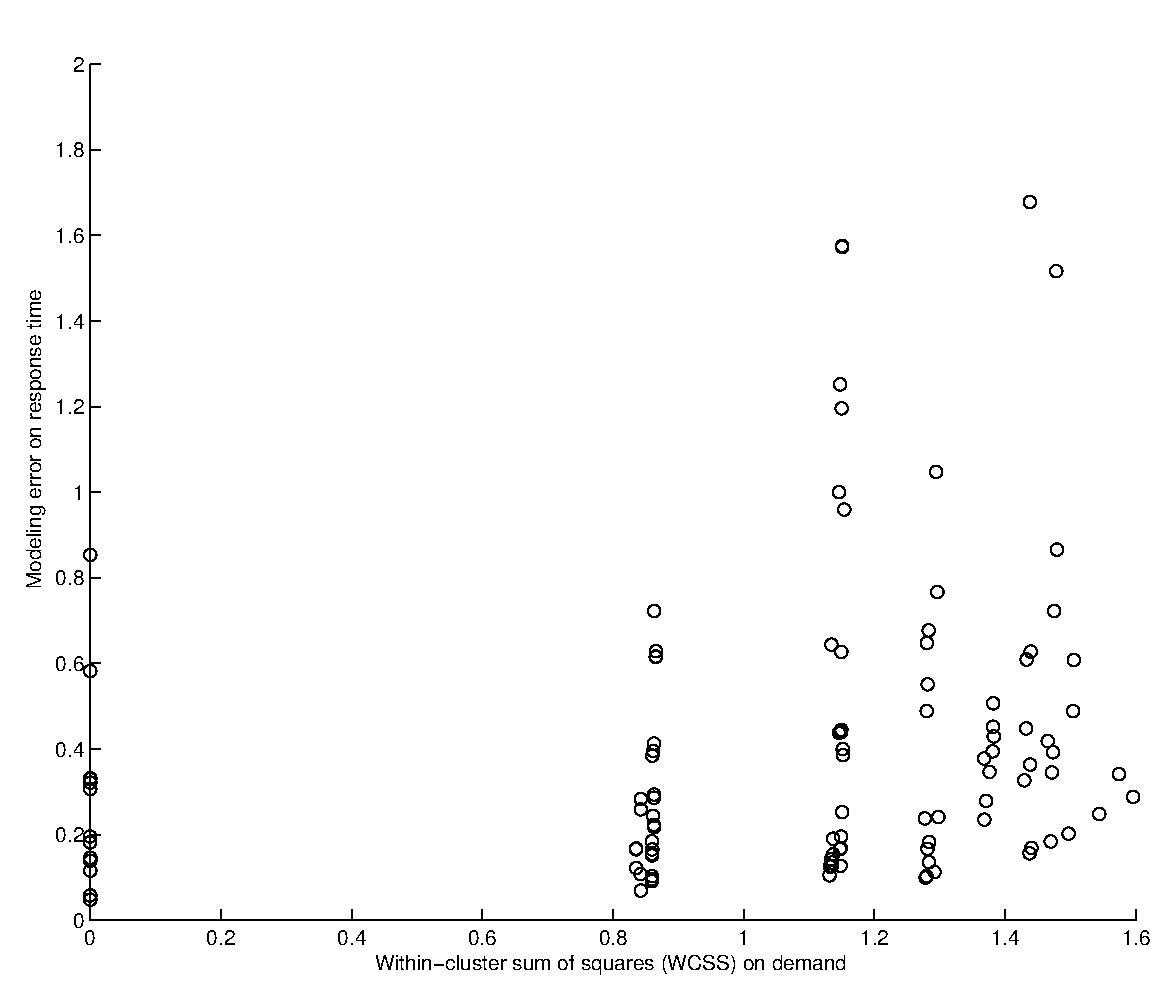
\includegraphics[width=0.7\textwidth]{image/clustering_error_corelation.eps} 
	\caption[The correlation between the within cluster sum-of-squares (WCSS) for demands and the modelling error.]{Correlation between the within cluster sum-of-squares (WCSS) for demands and the modeling error achieved on the response time's estimation.}
	\label{fig:cluster-sum-of-squares}
\end{figure}

\section{Estimation and Clustering for highly variable demands}  
Our TPC-W experiment covered a short interval; so the service demands did not vary a lot. As a result, it was unlikely that a class moved from one cluster to another. However, in the long run (e.g. a month in real system measures), classes might change place due to variation in the CBMG (and consequently service visits and service demands).   

A simulated experiment to investigate the effectiveness of the algorithm under non-uniform variations in demands was performed. This experiment showed the efficiency of the clustering and estimation for a web-based application where the estimated parameters change at different rates and phases. 
 The simulator software used was the CSim discrete event-based simulator. 
To keep the presentation simple but also to highlight the merits of the proposed method, in the simulation, we varied the think time $Z_c$ and the CPU demands, and kept $N_c$ constant.        


% This web-based application is an e-commerce site with 8 URLs (browse, buy, checkout, admin, login, logout, add, and remove). 
The system has 8 classes (c1-c8), two services (s1,s2), and two servers (w,d). Each service has only one replica, and each replica is placed on an individual server. Replicas are referred to as $j1$ and $j2$, or web and database.        
\begin{figure}[htbp]
	\centering
	%width=0.7\textwidth
   \includegraphics[ width=154mm, height=114mm]{image/image11.eps}
%	
\includegraphics[bb=0mm 0mm 208mm 296mm, width=84.8mm, height=68.7mm, viewport=3mm 4mm 205mm 292mm]{image/image12.eps}
	\caption[A sample service demands for 8 different classes on two services.]{Service demands for 8 different classes [c1,c2,c5,c6,c7,c8] on two services.
	}
	\label{fig:service-demands-different-classes}   
\end{figure}
 
 The classes are associated with a number of users ($N_c$), a mean user think time ($Z_c$), and time variant service demands $d_{c,\text{w}}$ and $d_{c,\text{db}}$. The service demands follow a sine curve with the same period, but different phases (see Figure \ref{fig:service-demands-different-classes}). Because of demand variations, classes migrate from one cluster to another, and the clusters evolve over time. In real applications, the service demands are not likely to change that dramatically, and we consider those variations as a stress load on the algorithm. Because of the variation of the service demands, we expect that the different classes will be re-clustered periodically.                                                                     

 Table \ref{tab:changes-clustering-structure} shows the clusters suggested by the K-means algorithm. The acceptable modeling error $A$ is set to 8\% over 421 simulation steps. The column `Action Nature' indicates the kind of change that has occurred when the past and current clusterings are compared. Ag, Br, Re, and Mv stand for aggregation, breaking, re-structuring, and movement respectively. The columns, "grouping (pre-event)" and "grouping (post-event)" represent the shape of the clusters before and after the re-clustering. % Note that in each re-clustering, the clusters are re-computed from scratch.  % ; meaning that the algorithm oblivious to `Action Nature.' 
\begin{table}
	\centering
\begin{tabular}{|p{0.3in}|p{0.8in}|p{2in}|p{2in}|} \hline 
Step & Action\newline Nature & Grouping\newline (Pre-event) & Grouping (Post-event) \\ \hline 
12 & Ag, Mv & [c1,c5,c6,c8] [c2,c7] [c3] [c4] & [c1,c2,c7,c8] [c3,c4]  [c5,c6] \\ \hline 
35 & Br & [c1,c2,c7,c8] [c3,c4] [c5,c6] & [c1,c2,c7,c8] [c3] [c4] [c5,c6] \\ \hline 
147 & Mv & [c1,c2,c7,c8] [c3] [c4] [c5,c6] & [c1,c5,c6,c8] [c2,c7][c3][c4] \\ \hline 
208 & Ag, Mv & [c1,c5,c6,c8] [c2,c7] [c3] [c4] & [c1,c2,c7,c8] [c3,c4] [c5,c6] \\ \hline 
239 & Br & [c1,c2,c7,c8] [c3,c4] [c5,c6] & [c1,c2,c7,c8] [c3] [c4] [c5,c6] \\ \hline 
340 & Mv & [c1,c2,c7,c8] [c3] [c4] [c5,c6] & [c1,c5,c6,c8] [c2,c7][c3][c4] \\ \hline 
400 & Br, Mv & [c1,c5,c6,c8] [c2,c7] [c3] [c4] & [c1,c2,c7] [c5,c6,c8] [c3,c4] \\ \hline 
\end{tabular}
	\caption[Changes in clustering the structure of user classes due to service demand change.]{Changes in clustering the structure of user classes due to service demand change.}
	\label{tab:changes-clustering-structure}  
\end{table}

Figure \ref{fig:tracked-demands}(a) shows the variation of the service demands in a changing cluster ([c2,c7]+[c1,c8]). Real and tracked service demands for the cluster are shown in Figure \ref{fig:tracked-demands}(b) while the modelling error is depicted in Figure \ref{fig:tracked-demands}(c). 
 \begin{figure}
	\centering
	\subfloat[][]{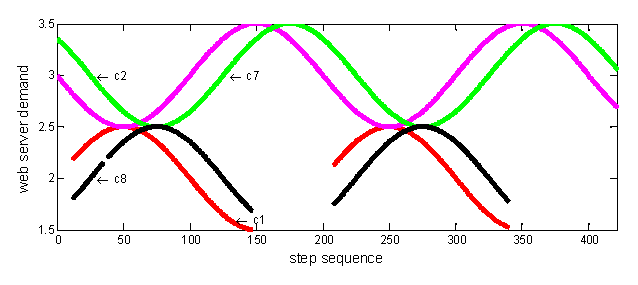
\includegraphics[width=0.6\textwidth]{image/variation-of-service-demands.eps}\label{fig:estimation-sub1}}  \\
	\subfloat[][]{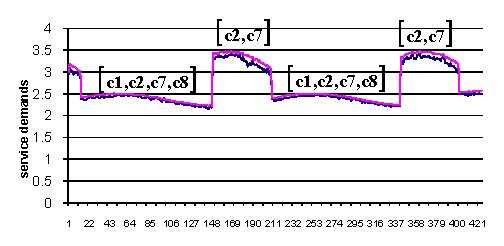
\includegraphics[width=0.6\textwidth]{image/real-and-tracked-service-demands2.eps}\label{fig:estimation-sub2}} \\
	\subfloat[][]{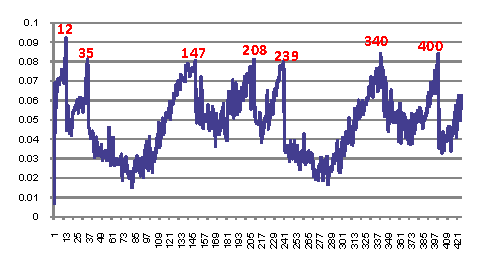
\includegraphics[width=0.6\textwidth]{image/the-modeling-error.eps}\label{fig:estimation-sub3}} \\
	\caption[An estimation case study: service demands, clusters, and modeling error.]
	{Represents (a) the variation of service demands,
		(b) real and tracked service demands for 2 clusters [c2,c7] and [c2,c7,c1,c8], 
		and (c) the modeling error with dynamic clustering applied.  }
	\label{fig:tracked-demands}
\end{figure}

According to Figure \ref{fig:tracked-demands}(a),  at step 50, $(d_{c1,\text{w}},d_{c1,\text{d}})$ and $(d_{c2,\text{w}},d_{c2,\text{d}})$ get close. This suggests that c1 and c2 should be in the same cluster near that step. At step 150, the service demands of c1 and c2 are quite different, indicating that these two classes are more likely in different clusters. These observations are consistent with our results where the clustering at step 50 is [c1,c2,c7,c8][c3][c4][c5,c6] and [c1,c5,c6,c8][c2,c7] [c3][c4] at step 150. Note that c1 and c8 are shown in Figure \ref{fig:tracked-demands}(a) only when they are part of the cluster [c2,c7,...]. This explains the step-function-like behaviour of the estimated demand for the changing cluster in Figure \ref{fig:tracked-demands}(b).

Based on Figure \ref{fig:tracked-demands}(c), during the simulation the modelling error exceeds the threshold A, 7 times. This means the classification algorithm described in Section III.B is activated 7 times among the 421 steps. One can see that not every re-clustering necessarily results into a different number of clusters. For example, at step 147, the clustering changes from [c1,c2,c7,c8][c3][c4][c5,c6] to [c1,c5,c6,c8][c3][c4][c2,c7]. The number of clusters remains the same, but c1 and c8 have been moved to a different cluster. Figure \ref{fig:number-clusters-over-time} shows that the total number of clusters changes only 4 times over the 400 steps.
\begin{figure}[h]
	\centering
	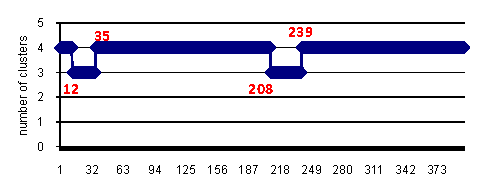
\includegraphics[width=0.7\textwidth]{image/number-clusters-versus-simulation-steps.eps}
	\caption[An estimation cases study: number of clusters over time.]{An estimation cases study: number of clusters over time.}
	\label{fig:number-clusters-over-time}
\end{figure}

We can conclude that our estimation and classification algorithm works quite well, since it is able to keep the error below $A$=0.08 with the smallest number of clusters and acceptable frequency of re-clustering. 

The algorithm also satisfies our claim: being able to exploit the complexity-accuracy trade-off and to keep both the modeling error and the monitoring and computational cost low. In terms of cost, our algorithm yielded half the required clusters (See Figure \ref{fig:number-clusters-over-time}) compared to full classes estimation, which from the theory reduces the estimation cost by a factor $2^3$ ($\frac{1}{2^3}$ of the original cost) and reduces the number of needed measurements by $4J$ (i.e. four fewer metrics for each replica). This is due to the fact that, the cost of the Kalman estimation in each step is dominated by Kalman gain calculation, which is $O(l^3)$ while $l$ is the number of measured variables. The reason is that the dominating term during gain calculation is an inversion of a matrix of size $l\times l$:
\begin{equation}
	K_n=P^-_nH^T_n{(H_nP^-_nH^T_n+\ R_n)}^{-1}
\end{equation} 
In this equation, $R_n$ is measurement noise covariance matrix with size $l\times l$.

In terms of accuracy, it was able to keep the error near zero compared to the case of fully aggregated classes. See Figure \ref{fig:comparison-of-modeling-error} for the error comparison between our algorithm, the one cluster case and the full classes estimation. 
\begin{figure}[h]
	\centering
	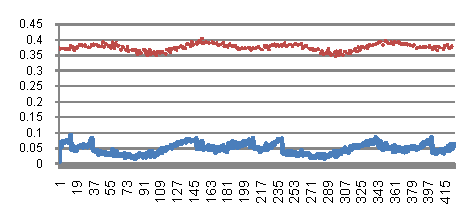
\includegraphics[width=0.7\textwidth]{image/comparison-modeling-error-one-cluster-dynamic.eps}
	\caption[Comparison of the modeling error for one cluster case, dynamic clustering case, and full classes estimation.]{Comparison of the modeling error for one cluster case (dotted line), dynamic clustering case (solid line), and full URLs estimation (solid horizontal line at $y=0$).}
	\label{fig:comparison-of-modeling-error}
\end{figure}

\section{Summary} 
\label{sec:conclusions-and-future-work} 
   Using Kalman filtering and LQM for hidden performance parameters estimation, is a promising approach. However, it introduces lots of monitoring overhead when the number of classes is increased. To mitigate this, we investigated a tracking approach, that identifies the performance parameters of groups of classes (we call them clusters) instead of individual classes. We proposed an algorithm that finds the appropriate number of clusters with a pre-defined clustering accuracy. 

We applied the clustering and tracking algorithm to two scenarios: 
(i) In the first experiment, we used our technique on the TPC-W benchmark deployed on a cluster of web servers. The workload was obtained from the well-known FIFA98 archives. In this experiment, first, we observed that the modelling error is reduced as the number of clusters increases. Second, we tested 140 different random ways to cluster the classes and computed their average error values ($E$). We observed that a clustering with a smaller average distance of classes to centroids (i.e., with smaller cluster sum-of-squares) has less error. Thus, we showed the usefulness of the K-means algorithm. Moreover, we dynamically computed the number of needed clusters that keep the modelling error under a threshold. For example, if one can accept 17\% error, the number of needed clusters for estimation would be dropped from 14 to 9 on average.
(ii) In the second experiment, we deployed our algorithm on a system with 8 classes. It was shown that our Extended Kalman filter could track hidden states successfully, and the correctness of the filter rose as it tried more classes and re-estimated service demands.

Our algorithm also satisfies our claim: being able to exploit the complexity-accuracy trade-off and to keep both the modeling error and the monitoring and computational cost low. 

In terms of cost, our algorithm yielded half the required clusters compared to full classes estimation, which from the theory reduces the estimation cost by a factor $2^3$ ($\frac{1}{2^3}$ of the original cost). 








